\chapter{Background} \label{ch:background}
\graphicspath{{Background/figures/}}

\section{Semantic Web} \label{sec:sematic-web}

The web can be seen as a worldwide, distributed system of interconnected documents that humans can read, exchange and discuss. The original model behind the web can be roughly summarized as a way to publish documents represented a standard way (e.g. HTML), containing links to other documents accessible through standard protocols (e.g. HTTP).

The great advantage of the web is that it abstracts the physical storage and network layers involved in the information exchange between machines. This enabled documents to appear directly connect to one another. However, in this paradigm machines are not able to achieve tasks based on automated data processing such as search and query answering. To overcome this limitation, research fields such as Information Retrieval (IR), Machine Learning (ML), and Natural Language Processing (NLP) produced complex systems trying to automatically extract meaning from unstructured data. A typical example would be search engines such as Yahoo\footnote{\url{http://www.yahoo.com}} and Google\footnote{\url{http://www.google.com}}. Despite their success, there is still a semantic gap between what the machine understands and how the user perceives the data~\cite{Mika:book:07}. This is where Semantic Web intervenes trying to fill the knowledge gap. In the same way that original Web abstracted away the network and physical layers, the Semantic Web abstracts away the document and application layers involved in the exchange of information. The Semantic Web connects facts, so that rather than linking to a specific document or application, you can instead refer to a specific piece of information contained in that document or application.Berners-Lee et al.~\cite{BernersLee:ScientificAmerican:01} provide the following definition for the Semantic Web:

\begin{quote}
\emph{The Semantic Web is not a separate Web but an extension of the current one, in which information is given well-defined meaning, better enabling computers and people to work in cooperation.}
\end{quote}

The word semantic itself implies meaning or understanding. The fundamental differences between Semantic Web and other data-related technologies is that the Semantic Web is concerned with the meaning and not the structure of data. This fundamental difference engenders a completely different outlook on how storing, querying, and displaying information might be approached.  Some applications, such as those that refer to a large amount of data from many different sources, benefit enormously from this feature.

What is meant by ``semantic'' in the Semantic Web is not that computers are going to understand the meaning of anything, but that the logical pieces of meaning can be mechanically manipulated by a machine to useful ends. For example, if a website publishes a database about a product line, with products and descriptions, while another publishes a database of product reviews. A third site for a retailer publishes a database of products in stock. The Semantic Web standards make it easier to write an application to mesh distributed databases together, so that a computer could use the three data sources together to help an end-user make better purchasing decisions.

Standards facilitate building applications, especially in a decentralized systems. To realize the Semantic Web vision, a series of technologies and standards have been proposed. We describe some of these standards in the following:

\subsection{Resource Description Framework (RDF)}
Resource Description Framework (RDF)~\cite{Lassila:RDF:99} is a recommendation of the World Wide Web Consortium (W3C) that describes the Web resources. It can be seen as the data modeling language for the Semantic Web.

Semantic Web resources can be anything that has an identity, they can be a person, document, image, location, etc. Each resource is assigned a Universal Resource Identifier (URI)~\cite{Berners:RFC:2005} which is a Unicode string to identify an abstract or physical resource. The most common type of URI is the Universal Resource Locator (URL) which is used to identify Web resources. A special case of a resource is a blank node for which no URI or literal is given. Blank nodes denote the existence of a resources with specific attributes but without providing any information about their identity or reference.

Resources can have atomic values named literal. They are simple Strings that describe data values that do not have a separate existence. They can be plain (simple string combined with an optional language tag (e.g. "thesis"@en)) or typed (string combined with a datatype URI and an optional language tag e.g. "0.99"\char`\^\char`\^datatypeURI). RDF reuses the  XML Schema (W3C) datatypes\footnote{\url{http://www.w3.org/TR/xmlschema-2}} which can be string, integer, float, double or date, as defined by the XML Schema Datatype specification.

RDF provides an intuitive knowledge representation using directed graphs, where the subjects and objects (resources) are the nodes and the predicates (properties) are the edges of that graph, this is referred to as an RDF Triple. Note that a property is a specific aspect, characteristic, attribute, or relation used to describe a resource~\cite{Lassila:RDF:1999}. Resources can be described and linked by other set of statements forming a larger graph or a semantic network. An atomic RDF statement is a triple which is usually denoted as $<s,p,o>$ and composed of:

\begin{itemize}
\item \textbf{Subject:} the URI of a resource or a blank node which the statement refers to.
\item \textbf{Predicate:} describes a property of the subject and expresses the relationship between the subject and the object.
\item \textbf{Object:} specifies the value of the property. It can be a URI of a resource, blank node or a literal.
\end{itemize}

Figure~\ref{fig:rdfGraph}~\info{Do i have to reference the image?} depicts an example of RDF graph-based representation for an address. An address is a structure that consists of different values such as a street, a city, a state and a zipcode.

 \begin{figure}[htbp]
   \centering
  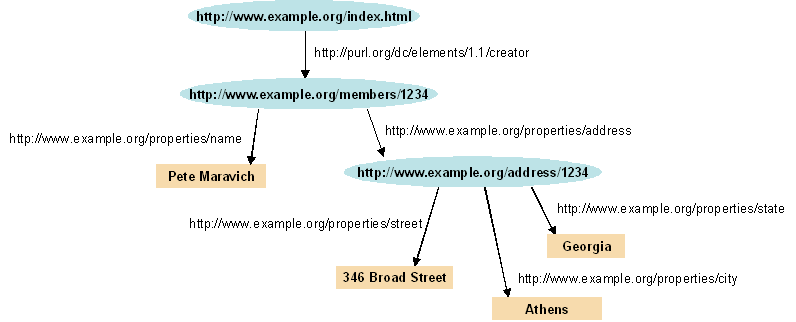
\includegraphics[width=\linewidth]{rdf.png}
  \caption{Example of RDF representation of an addres}
  \label{fig:rdfGraph}
  \end{figure}

Several methods exist for serializing the RDF data model. The most common format is RDF/XML. There exist other text-based formats introduced by W3C such as Turtle\footnote{\url{http://www.w3.org/TeamSubmission/turtle}} and N-Triples\footnote{\url{http://www.w3.org/TR/n-triples}} which are easier to read than RDF/XML.

RDF also contains data structures (containers and collections) that allow aggregating nodes or facts together. They are basically a syntactic sugar that will ease the process of writing code with no semantic expressiveness whatsoever.

\subsection{RDF Schema}

\begin{flushright}
\textit{``It's impossible to get everyone everywhere to agree on a single label for every specific thing that ever was, is, or shall be''}\\
Cambridge Semantics~\cite{Cambridge:RDF-101:13}
\end{flushright}

RDF is a very simple and flexible data model that allows users to describe resources using properties and values. However, it does not provide means to define vocabularies and to specify domain specific classes and properties. Hence, other terms are needed to describe the classes of resources and the relationship between them. As a solution, an extension of RDF called RDF Schema~\cite{Brickley:2014} provides a basic vocabulary to interpret RDF statements. RDFS vocabulary simply describes taxonomies of classes and properties and defines very basic restrictions.

In RDF Schema, URIs have as a namespace \url{http://www.w3.org/2000/01/rdf-schema#}
conventionally associated with the prefix \emph{rdfs:}. In summary, (1) A resource is an instance of one class (\emph{rdfs:class}) or more classes where classes are organized in a hierarchy using \emph{rdfs:subClassOf} property; (2) Properties have as class \emph{rdf:Property} and are organized in a hierarchy using \emph{rdfs:subPropertyOf}. Some restrictions on properties are specified such as \emph{rdfs:domain} to define the class of the subject, and \emph{rdfs:range} to define the class of the object.

\subsection{Ontology Vocabulary}
RDF and RDF Schema both have limited expressivity. While RDF describes a simple way to represent structured data, RDF Schema only provides basic hierarchies associated with simple restrictions. However, there is a need for more expressivity to be able to define a formal explicit description of concepts in some complex domains. Therefore, the concept of ontology has been adopted as an extension of RDF Schema with more expressive constructs. Ontology was originally defined by Artificial Intelligence (AI) community as explicit formal specification of a conceptualization in domain of interest~\cite{Gruber:1993}. It typically describes the concepts of the domain and the semantic interconnections that hold between them, along with some logic and inference rules. In general, ontology is the reflection of a shared and common  understanding of a domain that can be communicated between people and/or machines. For example, given the different websites containing event information, the use of common ontology will enable Web agents to aggregate data and to answer more complex user queries. In the following, we list some core elements of an ontology:

\begin{itemize}
\item Class: defines a concept, type or collection in a specific domain. It groups objects that share some properties and are organized in a hierarchy. For instance, in a university domain, the class Student is more specialized than the class Person.
\item Individual: also known as instance or object and is a member of a class. For instance, \emph{Nelson Mandela} is an instance of the class Person.
\item Property: is a binary relation to describe how classes and individuals can be related to each another. There is datatype property which connects instances with RDF literals, and object property which connects instances of two classes. For example, \emph{hasFather} is an object property that can relate two instances of the class Person.
\end{itemize}

To model ontologies, the Web Ontology Language (OWL)~\cite{OWL:2012} is the current markup language endorsed by W3C. Compared with RDF and RDFS, OWL defines a vocabulary with additional formal semantics. It provides more relations between classes (e.g. \emph{disjointWith}), logical properties (e.g. \emph{intersectionOf}, \emph{sameAs}) and enumerations (e.g. \emph{oneOf}, \emph{allValuesFrom}), among others.

\subsection{SPARQL Query Language}

Given that now we have our data modeled as RDF, it is now possible to query and ask questions about these facts in a very powerful way. For that, we have SPARQL as a query language

To query the RDF graph, W3C has defined a query language called SPARQL\footnote{\url{http://www.w3.org/TR/rdf-sparql-query}}. It contains triple patterns along with their conjunctions (e.g. logical ``and'') and disjunctions (e.g. logical ``or''). It also supports extensible value testing and constraining queries by named RDF graph.


\subsection{Linked Open Data}

The Semantic Web is predicated on the availability of large amount of structured RDF data, not in isolated islands but as a Web of interlinked data. A major milestone to realize this vision is the Linked Open Data (LOD or Linked Data) project~\cite{LOD:2011} that connects RDF datasets on a large scale. LOD captures a growing knowledge from various domains forming an open ``Web of Data'' freely available to access, download, and use. Today's LOD comprises billions of RDF triples counting millions of links between data sources. Formally, Linked Data has been defined as about ``data published on the Web in such a way that it is machine readable, its meaning is explicitly defined, it is linked to other external datasets, and can in turn be linked to from external datasets''~\cite{Bizer:HB09}.

Linked Data follows the principles outlined by Tim Berners-Lee to publish information on the Web, which are:

\begin{itemize}
\item Use URIs as names for things
\item Use HTTP URIs so that people can look up those names.
\item When someone looks up a URI, provide useful information, using the standards (RDF, SPARQL)
\item Include links to other URIs. so that they can discover more things.
\end{itemize}

Overall, these principles stress on the accessibility and the linkage of data that adhere to the architecture and standards of the Web. Figure~\ref{fig:lod} shows the significant number of published datasets in 2011, covering information from diverse areas such as encyclopedic, government, geographic, entertainment, publications and so on.  For instance, DBpedia\footnote{http://dbpedia.org} is one of the largest RDF repository in the Linked Data focusing on extracting multilingual knowledge from Wikipedia. At the time of writing, the English edition of DBpedia consists of 470 millions RDF triples that describe 4.0 million things covering a wide range of topics, and contains 45 million RDF links to several hundred external datasets.

 \begin{figure}[htbp]
   \centering
  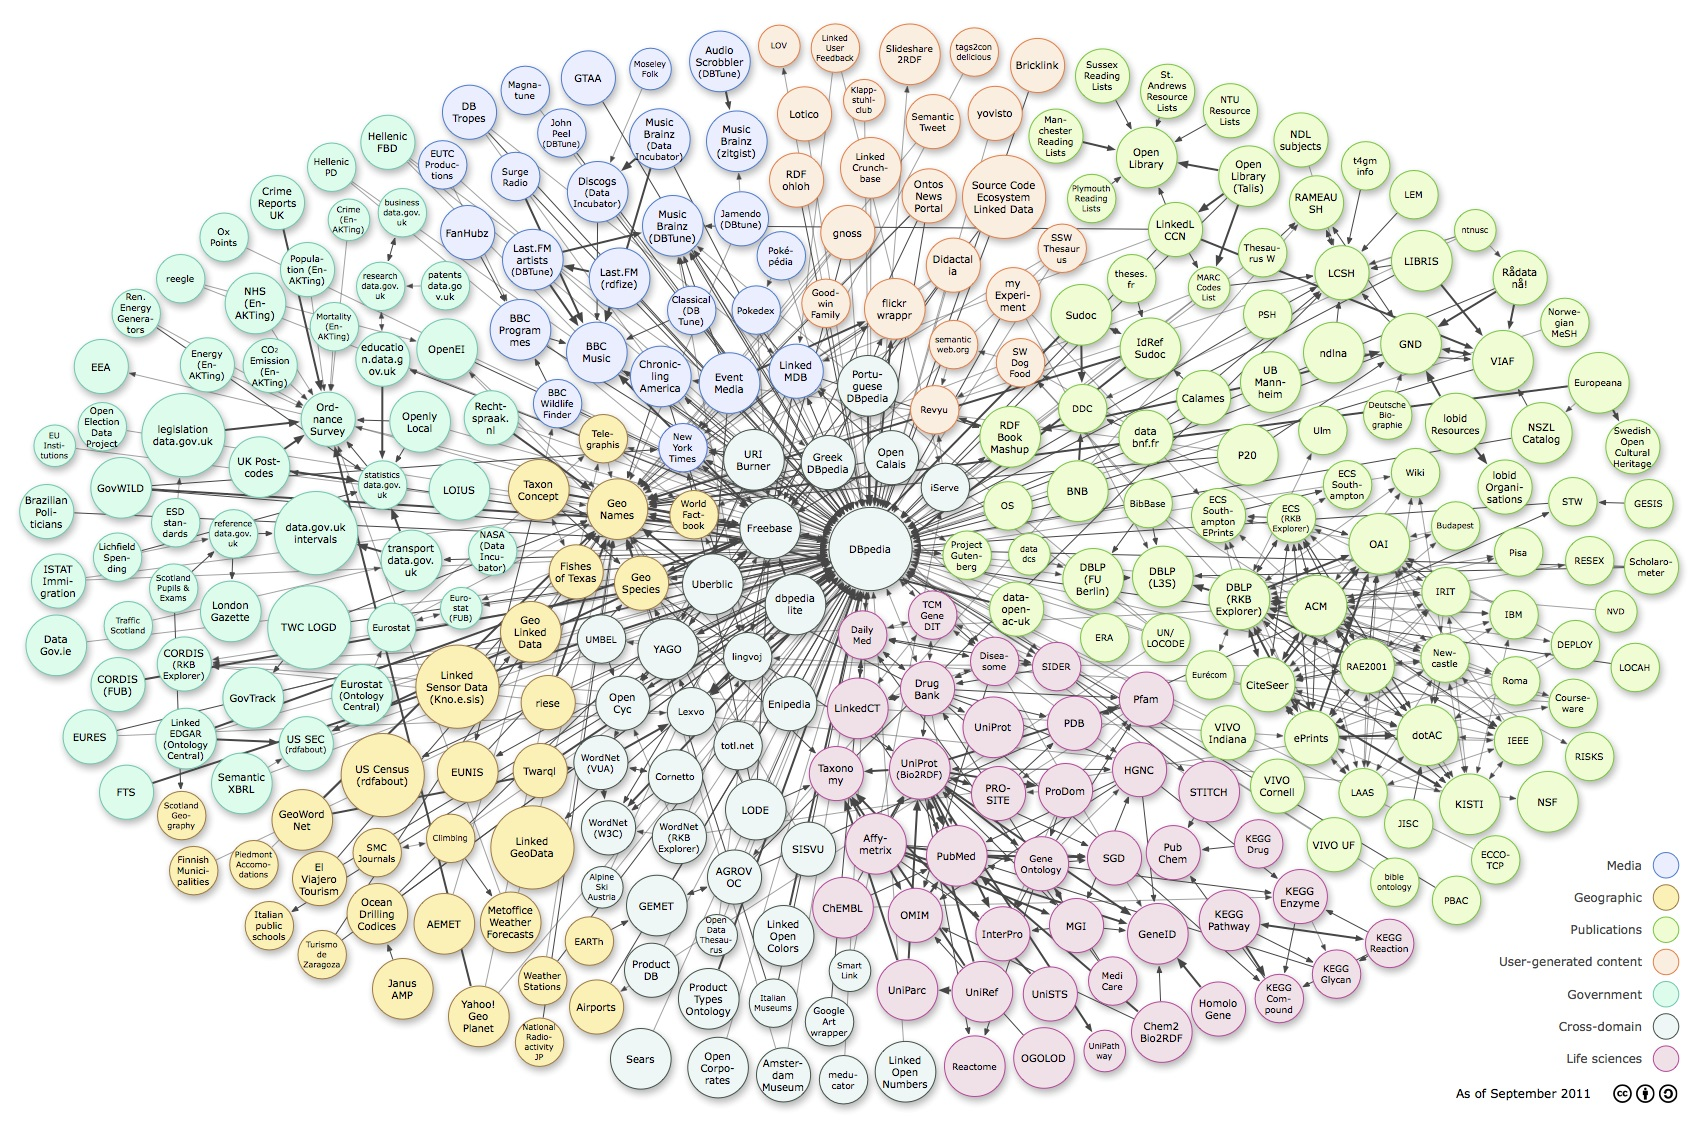
\includegraphics[width=\linewidth]{lod.jpg}
  \caption{Linked Open Data (LOD) Cloud in September 2011}
  \label{fig:lod}
 \end{figure}

Client applications can access and use RDF links to navigate between datasets and to discover additional information. In order to be part of Linked Data, datasets need to create links to related instances in other datasets. To cope with the large amount of instances, it is a common practice to draw on automated or semi-automated tools or methods to generate links between data sources. Yet, this is still a challenging task and significant research efforts have been devoted to address it.


